\section{稳定性：循环模型首先是一个动态系统}
\label{sec:stability-dynamical-system}

本章的核心判断是：循环 Transformer（Loop Transformer）一旦把同一个共享模块反复作用在隐藏状态上，它就已经进入动态系统（dynamical system）问题域。性能能否随着递归深度增加而改善，先取决于状态轨迹能否保持可控；如果残差流（residual stream）里的隐藏状态范数失控，后续所有“内部思考”的解释都会失去基础。

\begin{importantbox}{本章主张}
循环模型的第一道硬门槛是稳定性。递归深度带来额外计算，也带来误差放大、状态偏移和损失脉冲；约束与归一化的作用，是让每次更新都在可控范围内推进。
\end{importantbox}

\subsection{从递归深度到动态系统}

前一章把递归深度解释成测试时计算的调节器：模型可以在推理时多运行几轮共享块，让隐藏状态获得更多更新机会。本章要补上一层更底层的事实：同一个函数被重复调用时，微小偏差会沿着递归链条传播。若每一步都把状态推离稳定区域，循环次数越多，模型越容易把可用表示放大成噪声。

视频在 00:07:03--00:07:40 强调了这个问题：循环架构从一串彼此独立的层，转为对隐藏状态重复应用相同变换；此时需要决定循环次数，并确保信息不会在反复更新中变得混乱。直观类比是反复调整同一份草稿：每次修改都可能让表达更清楚，也可能把前一步的小误差扩成整段文字的偏题。模型内部也类似，只是草稿从文本变成了连续向量。

先用朴素语言说公式要表达的内容：隐藏状态 \(h_t\) 是第 \(t\) 次递归后的内部表示；下一轮状态由旧状态经过同一个更新规则得到，同时混入输入信息。画面中的简化形式把复杂的 Transformer 更新线性化为两部分：旧状态的传播和输入的注入。

\[
h_{t+1}=Ah_t+Bx
\]

符号说明：
\begin{itemize}
  \item \(h_t\)：第 \(t\) 次递归后的隐藏状态，也就是模型当前的内部工作记忆。
  \item \(h_{t+1}\)：下一次递归后的隐藏状态。
  \item \(A\)：旧隐藏状态如何被继续传播和变换的简化矩阵。
  \item \(B\)：输入 \(x\) 如何被注入当前状态的简化矩阵。
  \item \(x\)：当前 token 或上下文输入提供的信息。
\end{itemize}

这个式子只是讲义层面的线性化直觉。真实的 Transformer 块包含 attention、MLP、归一化和残差连接，通常可以写成更一般的共享更新：

\[
h_{t+1}=F_\theta(h_t,x)
\]

符号说明：
\begin{itemize}
  \item \(F_\theta\)：被反复复用的 Transformer 递归模块，\(\theta\) 是共享参数。
  \item \(h_t\)：递归前的隐藏状态。
  \item \(x\)：输入信息或注入到循环中的上下文表示。
  \item \(h_{t+1}\)：应用同一模块后得到的新状态。
\end{itemize}

\begin{figure}[htbp]
  \centering
  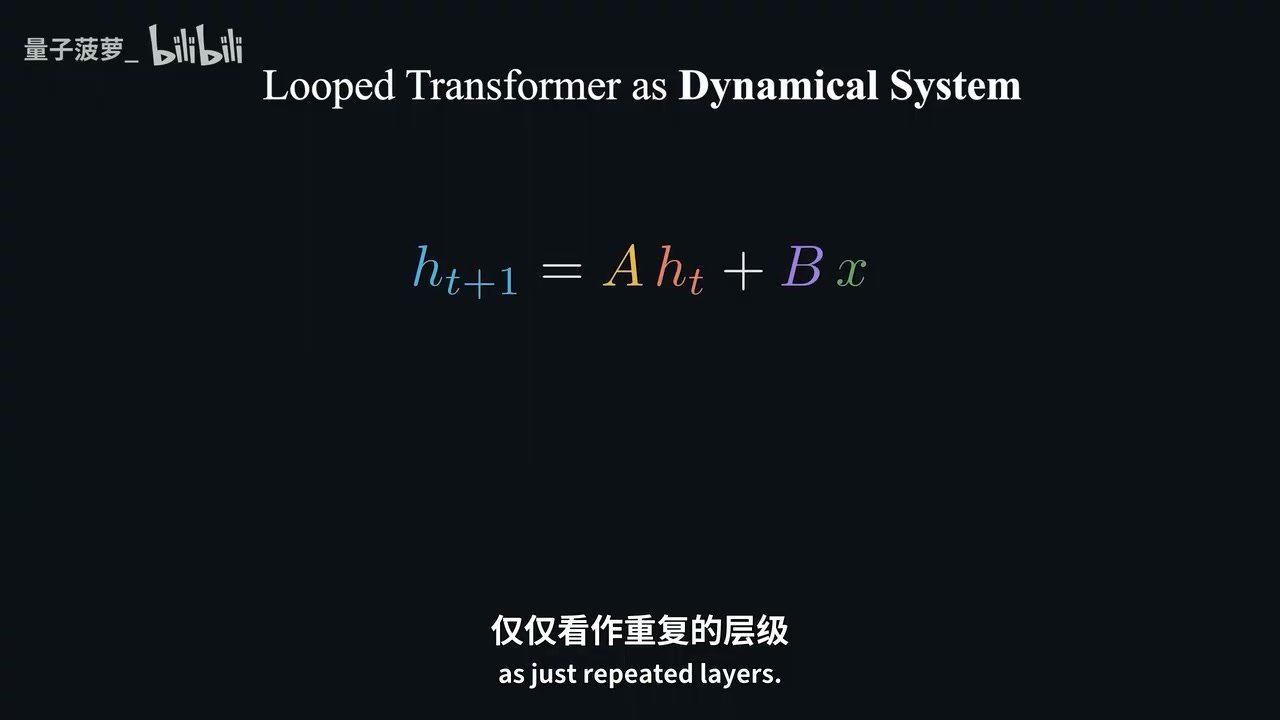
\includegraphics[width=0.82\linewidth,height=0.36\textheight,keepaspectratio]{figures/fig_07_dynamical_system_equation.jpg}
  \caption{循环 Transformer 被视为动态系统后，隐藏状态更新可以用 \(h_{t+1}=Ah_t+Bx\) 这样的简化形式建立直觉。\protect\footnotemark}
  \label{fig:residual-stream-dynamics}
\end{figure}
\footnotetext{视频画面时间区间：00:07:43--00:07:52。}

\subsection{残差流为什么成为状态主通道}

动态系统视角之所以落在残差流上，是因为残差流承载了 Transformer 层间持续传递的信息。标准深层 Transformer 中，每一层都有自己的参数，残差流像一条主干河道，沿途接受不同支流的注入。循环 Transformer 中，主干河道依旧存在，只是同一套处理装置被反复接到河道上；每一轮都读取旧状态、混入输入、执行 Transformer 操作，再把结果写回残差流。

视频在 00:07:52--00:08:15 说明了这个机制：隐藏状态每次出现都会向前传播并更新，而非从头重新计算；每次循环都会重用之前的隐藏状态，并与注入输入混合。因此，残差流本质上就是递归过程里的潜在状态（latent state）。如果这个通道有序，递归可以逐步整合信息；如果这个通道失控，递归只会把混乱带到下一轮。

为了说明稳定更新，讲义可以把残差更新写成“旧状态加上本轮修正，再做归一化”。这条公式表达的是：循环块不应每轮重造一个全新状态，而应在旧状态上追加受控修正。

\[
h_{t+1}=\mathrm{Norm}\bigl(h_t+\Delta_\theta(h_t,x)\bigr)
\]

符号说明：
\begin{itemize}
  \item \(h_t\)：进入第 \(t+1\) 次递归前的残差流状态。
  \item \(\Delta_\theta(h_t,x)\)：共享模块根据当前状态和输入产生的本轮修正量。
  \item \(h_t+\Delta_\theta(h_t,x)\)：残差式累积，表示旧状态被保留并被更新。
  \item \(\mathrm{Norm}(\cdot)\)：归一化或约束操作，用来限制尺度漂移。
  \item \(h_{t+1}\)：归一化后的下一轮状态。
\end{itemize}

\begin{knowledgebox}{稳定性直觉}
从第一性原理看，循环模型的危险来自“反复乘上同一个变化”。若某个方向上的更新每轮都会把向量长度放大 \(1.1\) 倍，十几轮后就会形成明显漂移；若更新被约束在稳定范围内，递归才可能像迭代求解器一样逐步逼近有用表示。
\end{knowledgebox}

\subsection{隐藏状态范数、损失脉冲与发散}

稳定性最容易观察的信号之一是隐藏状态范数（hidden-state norm）。范数可以理解为向量“有多大”：它不直接告诉读者状态里的语义是否正确，却能提醒读者状态尺度是否正在失控。视频在 00:08:15--00:08:27 指出：如果动态系统不稳定，隐藏状态的范数会在递归中增长，引发训练损失（training loss）的脉冲和发散；约束与归一化的任务，就是防止每次更新因为不受控累积而崩溃。

先用白话解释下面的量：若模型每轮更新都让 \(\lVert h_t\rVert\) 变大，训练损失 \(L_t\) 往往会出现突增。这个突增并不神秘，它常常意味着模型内部状态进入了训练过程很难处理的尺度范围。

\[
\lVert h_{t+1}\rVert \le \alpha \lVert h_t\rVert+\beta \lVert x\rVert,\qquad 0\le \alpha \lesssim 1
\]

符号说明：
\begin{itemize}
  \item \(\lVert h_t\rVert\)：第 \(t\) 次递归后隐藏状态的范数，表示状态尺度。
  \item \(\lVert h_{t+1}\rVert\)：下一轮状态尺度。
  \item \(\alpha\)：旧状态在下一轮中被放大的程度；接近或低于 \(1\) 更利于稳定。
  \item \(\beta\)：输入信息对状态尺度的影响强度。
  \item \(\lVert x\rVert\)：输入表示的范数。
\end{itemize}

这里的关键是稳定性约束的方向：旧状态的影响不能无限放大，输入注入也要有边界。对工程实现来说，这通常会落到 normalization、residual scaling、门控、训练初始化和递归步数策略上。

\begin{figure}[htbp]
  \centering
  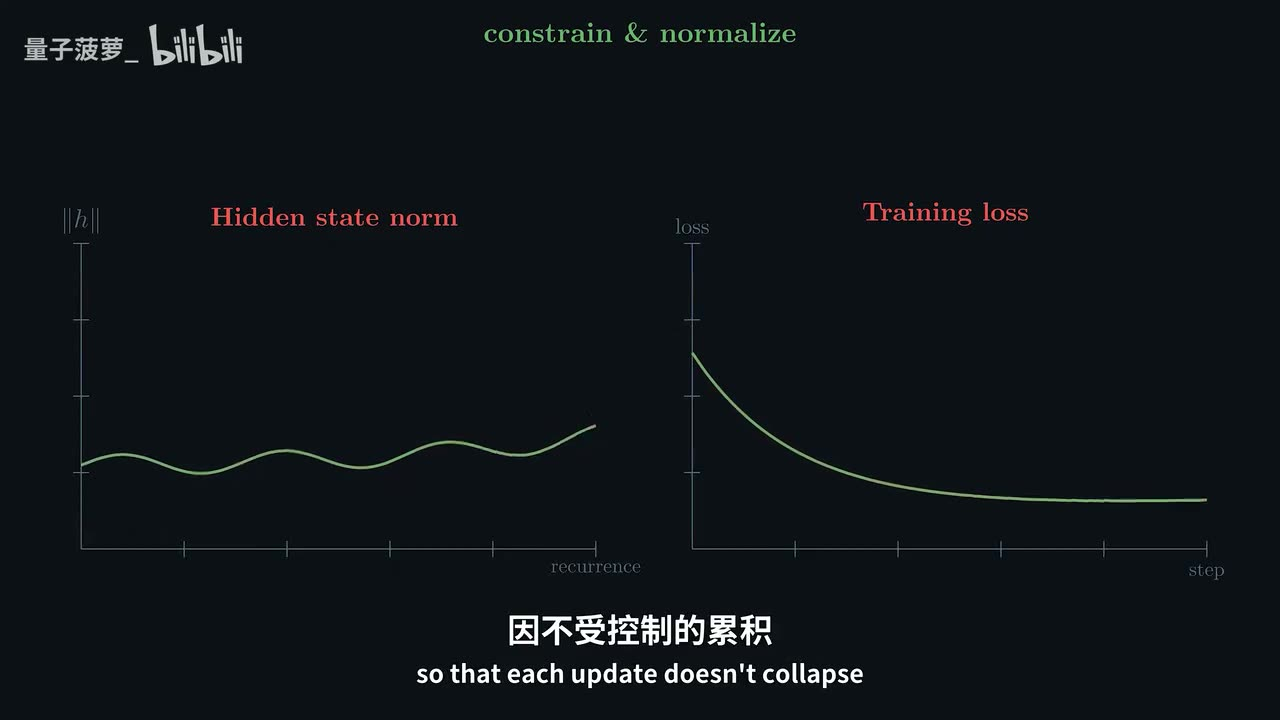
\includegraphics[width=0.82\linewidth,height=0.36\textheight,keepaspectratio]{figures/fig_08_instability_norm_loss.jpg}
  \caption{约束与归一化用于限制隐藏状态范数的失控增长，从而减少训练损失中的脉冲和发散风险。\protect\footnotemark}
  \label{fig:instability-norm-loss}
\end{figure}
\footnotetext{视频画面时间区间：00:08:20--00:08:30。}

\subsection{固定点和周期：下一章证据的预备概念}

一旦把循环模型看成动态系统，读者自然会问：反复更新最后会去哪里？有三种典型结局。第一种是趋近固定点（fixed point），状态越来越接近某个稳定位置；第二种是进入周期轨迹（cycle），状态在若干个区域之间有规律地来回访问；第三种是发散，状态尺度或方向不断失控。前两种至少说明系统存在结构，第三种通常意味着模型难以可靠使用。

固定点的直觉是：再更新一轮，状态也几乎不变。

\[
h^\star \approx F_\theta(h^\star,x)
\]

符号说明：
\begin{itemize}
  \item \(h^\star\)：递归过程趋近的稳定隐藏状态。
  \item \(F_\theta\)：共享递归模块。
  \item \(x\)：输入或上下文信息。
  \item \(\approx\)：表示近似相等，实际模型中通常只能观察到接近稳定。
\end{itemize}

周期轨迹的直觉是：状态隔 \(p\) 轮后回到相似区域。

\[
h_{t+p}\approx h_t
\]

符号说明：
\begin{itemize}
  \item \(t\)：当前递归步。
  \item \(p\)：周期长度，表示经过多少轮后回到相似状态。
  \item \(h_{t+p}\)：第 \(t+p\) 次递归后的状态。
  \item \(h_t\)：第 \(t\) 次递归后的状态。
\end{itemize}

\begin{warningbox}{稳定性证据边界}
稳定轨迹只说明递归过程没有明显乱跑或崩溃。它还不能直接证明模型学会了人类可解释的推理算法。下一章的机制证据必须继续追问：这些轨迹是否和注意力行为、推理阶段、答案收敛相互呼应。
\end{warningbox}

\subsection{本章小结}

本章把 Loop Transformer 从“重复运行几层”推进到“在残差流上定义动态系统”。读者应带走三个判断：第一，递归深度带来计算机会，也放大稳定性风险；第二，残差流是隐藏状态前后传递的主通道，归一化和约束是在保护这条通道；第三，固定点和周期轨迹是观察内部递归结构的入口，真正的机制解释还需要结合下一章的 PCA、注意力稳定和阶段化递归证据。
